\documentclass[11pt,a4paper]{article}
\usepackage[utf8]{inputenc}
\usepackage{amsmath,enumitem,amsfonts,amssymb,graphicx,commath}
\usepackage{sectsty}
\usepackage{multicol}
\usepackage{tikz}
\usepackage{graphicx}
\usetikzlibrary{shapes,arrows,automata,arrows.meta}

\graphicspath{ {./img/} }
\DeclareMathAlphabet{\pazocal}{OMS}{zplm}{m}{n}

\usepackage[%
    left=1in,%
    right=1.0in,%
    top=0.8in,%
    bottom=1in,%
]{geometry}%

\sectionfont
{\fontsize{14.4}{12}\selectfont}
\title{\textbf{Principles of AI Planning
		\\{\Large Exercise Sheet 13}}}
\makeatletter
\renewcommand{\@maketitle}
{
	\newpage
	\null
	\vskip 2em%
	\begin{center}%
		{\LARGE \@title \\ \par}%
	\end{center}%
	\par
} \makeatother

\begin{document}
\begin{flushleft}
	Authors:\\
	Erick Rosete Beas | er165@uni-freiburg.de\\
	Jessica Lizeth Borja Diaz | jb986@uni-freiburg.de\\
\end{flushleft}
{\let\newpage\relax\maketitle}
\begin{center} 
	\large 07.02.2020
\end{center}


%%%%%%%%%%%%%%%%%%%%%  Ejercicio 1 %%%%%%%%%%%%%%%%%%%%%%%%%
\section*{Exercise 13.1 - EVMDDs}
(a)
\begin{center}
	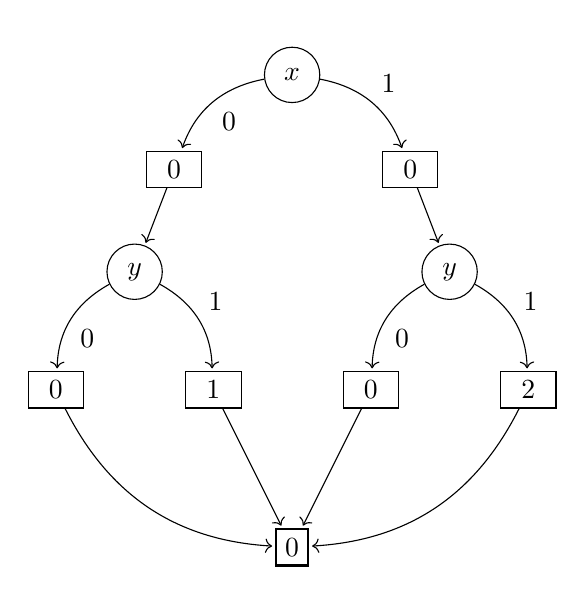
\begin{tikzpicture}
		\begin{scope}
            [
                styleVar/.style={
					minimum width = 2em, draw, circle,
					label={[above]#1}
					},
				styleCost/.style={minimum width = 2em, draw},
				end/.style={ minimum width = 0.2em, draw, thick},
            ]
			\node(x)[styleVar] at (0,0) {$x$};
			\node(cx0)[styleCost] at (-1.5,-1.2) {$0$};
			\node(cx1)[styleCost] at (1.5,-1.2) {$0$};

			\node(y)[styleVar] at (-2,-2.5) {$y$};
			\node(cy0)[styleCost] at (-3,-4) {$0$};
			\node(cy1)[styleCost] at (-1,-4) {$1$};
			
			\node(yp)[styleVar] at (2,-2.5) {$y$};
			\node(cyp0)[styleCost] at (1,-4) {$0$};
			\node(cyp1)[styleCost] at (3,-4) {$2$};

			\node(end)[end] at (0,-6){$0$};
		\end{scope}
		\begin{scope}
            [->=stealth',shorten >=1pt,auto]
            \path 
			(x) edge[bend right]        node{$0$}(cx0)
			(x) edge[bend left]         node{$1$}(cx1)
			(cx0) edge     				node{}(y)
			(cx1) edge			     	node{}(yp)

			(y) edge[bend right]        node{$0$}(cy0)
			(y) edge[bend left]         node{$1$}(cy1)
			(cy0) edge[bend right]      node{}(end)
			(cy1) edge				    node{}(end)

			(yp) edge[bend right]        node{$0$}(cyp0)
			(yp) edge[bend left]         node{$1$}(cyp1)
			(cyp0) edge      		     node{}(end)
			(cyp1) edge[bend left]       node{}(end);

		\end{scope}
    \end{tikzpicture}
\end{center}

%%%%%%%%%%%%%%%%%%%%%  Ejercicio 2 %%%%%%%%%%%%%%%%%%%%%%%%%
\section*{Exercise 13.2 - Evaluating states with EVMDDs}


%%%%%%%%%%%%%%%%%%%%%  Ejercicio 3 %%%%%%%%%%%%%%%%%%%%%%%%%
\section*{Exercise 13.3 - EVMDD sizes and variable orders}
Consider a cost function represented by the EVMDD on the right.\\
Let $s$ be a state with $s(x) = 1$ and $s(y) = 2$. To which value does the
EVMDD evaluate for state $s$?\\
$cost(s) = 3 + 0 + 5 = 8$
\begin{figure}[h!]
	\centering
	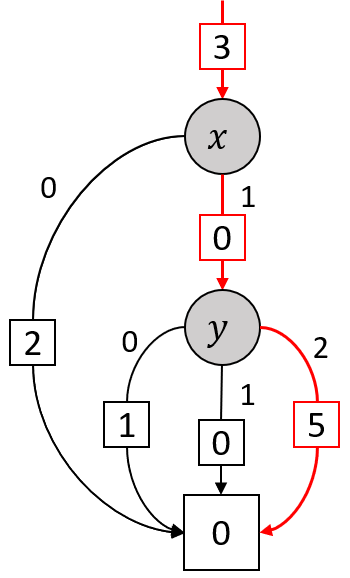
\includegraphics[scale=0.5]{13_3.png}
\end{figure}
%%%%%%%%%%%%%%%%%%%%%  Ejercicio 4 %%%%%%%%%%%%%%%%%%%%%%%%%
\section*{Exercise 13.4 - EVMDD-based action compilation}
Consider again the EVMDD from Exercise 13.3. Assume it encodes the cost $c_{o_1}$ of operator $o_1 = \langle z = 1 \land u = 1, x := 0\rangle$.

\begin{enumerate}[label=\alph*)]
	\item Give the EVMDD-based action compilation of $o_1$ using this EVMDD.
	\begin{align*}
		&O_1^{z=1 \land u=1} = \langle z = 1 \land u = 1 \land \sigma = 0 \land \alpha_{o_1} = 0, \sigma := 1 \land \alpha_{o_1} = 1\rangle & cost=3&\\
		&O_1^{1, x=0} = 
	\end{align*}
\end{enumerate}
\end{document}